\documentclass{article}
%\usepackage{ctex}
\usepackage{amsfonts,amssymb,amsmath}
\usepackage{graphicx}

\begin{document}

\title{{\bf Review Automata Theory}}
\author{{\bf [ quant67 ]}\\
Harbin Engineering University\\}
\date{\today}
\maketitle

\section{Why Study the Theory of Computation?}

$\cdots$

No reason for me.

\section{Languages and Strings}

\subsection{Strings}

A string is a finite sequance, possibly empty, of symbols drawn from alphabet $\Sigma$. Note that $\varepsilon$ is an empty string and that $\Sigma^*$ is the set of all possible strings over an alphabet $\Sigma$.

\subsubsection{Functions on Strings}

\begin{description}
  \item[$|s|$:] the length of a string s.
  \item[$\#_c(s)$:] the number of times that the symbol c occurs in s.
  \item[st:] the concatenation of two strings s and t, also written $s||t$.
  \item[$w^i$:] the replication of string w. $w^0=\varepsilon, w^{i+1}=w^iw$.
  \item[$w^R$:] string reversal. $(wx)^R=x^Rw^R$.
\end{description}

\subsubsection{Relations on Strings}

A string s is a {\bf substring} of a string t iff s occurs contiguously as part of t.

A string s is a {\bf proper substring} of a string t iff s is a substring of t and $s\not=t$.

A string s is a {\bf prefix} of t iff $\exists x\in\Sigma^*(t=sx)$. A string s is a {\bf proper prefix} of a string t iff s is a prefix of t and $s\not=t$.

A string s is a {\bf suffix} of t iff $\exists x\in \Sigma^*(t=xs)$. A string s is a {\bf proper suffix} of a string t iff s is a suffix of t and $s\not=t$.

\subsection{Languages}

A {\bf language} is a (finite or infinite) set of strings over a finite alphabet $\Sigma$.

If $\Sigma\not=\phi$ then $\Sigma^*$ is countably infinite.

If $\Sigma\not=\phi$ then the set of languages over $\Sigma$ is uncountably infinite.

$L_1L_2=\left\{ w\in\Sigma^* : \exists s\in L_1 (\exists t \in L_2(w=st)) \right\}$. $(L_1L_2)L_3 = L_1(L_2L_3)$.

$L^*=\left\{ \varepsilon \right\}\cup \left\{ w\in \Sigma^*: \exists k\ge 1 ( \exists w_1,w_2,\cdots ,w_k \in L (w=w_1w_2\cdots w_k ) ) \right\}$.

$L^+=LL^*$.

$L^R=\left\{ w\in \Sigma^*: w=x^R\ for\ some\ x \in L \right\}$, $(L_1L_2)^R=L_2^RL_2^R$.

\section{The Big Picture: A Language Hierarchy}

\begin{figure}[h]
\centering
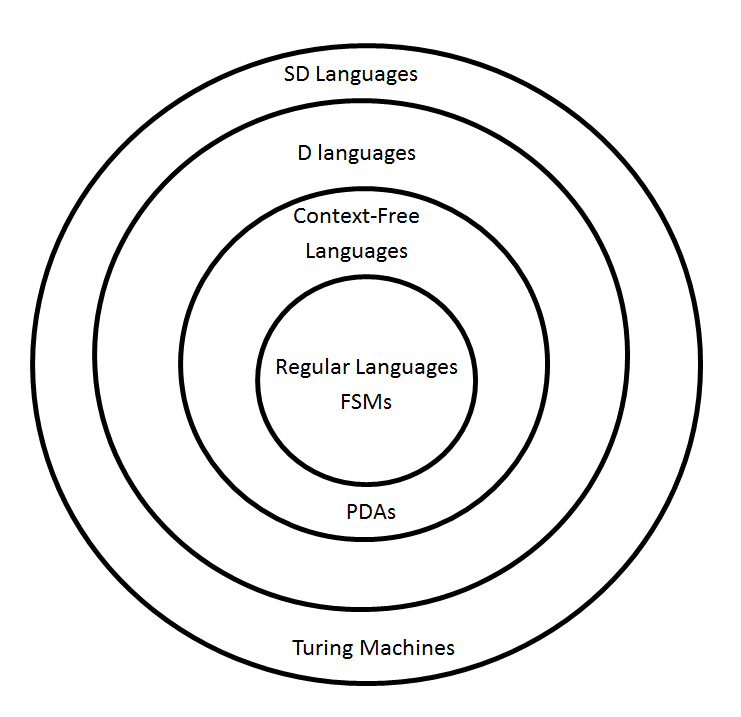
\includegraphics[height=6.7cm]{hierarchy.png}
\caption{A hierarchy of language classes}
\end{figure}

\section{Computation}

Nothing to care about here, or it is hard to say.

\section{Finite State Machines}

\subsection{Deterministic Finite State Machines}

A {\bf deterministic FSM}(or {\bf DFSM}) M is a quintuple $(K, \Sigma, \delta, s, A)$, where:
\begin{itemize}
  \item K is a finite set of states,
  \item $\Sigma$ is the input alphabet,
  \item $s\in K$ is the start state,
  \item $A\subseteq K$ is the set of accepting states, and
  \item $\delta$ is the transition function. It maps from $K\times \sigma\ to\ K$.
\end{itemize}


M accepts w iff $(s, w)|-_M^*(q, \varepsilon)$, for some $q\in A_M$, Any configuration $(q, \varepsilon)$, for some $q\in A_M$, is called an accepting configuration of M.

M rejects w iff $(s, w)|-_M^*(q, \varepsilon)$, for some $q\not\in A_M$, Any configuration $(q, \varepsilon)$, for some $q\not\in A_M$, is called a rejecting configuration of M.

\subsection{The Regular Languages}
We define the set of {\bf regular languages} to be exactly those that can be accepted by some DFSM.

\subsection{Nondeterministic FSMs}
also called {\bf NDFSM}.

\subsubsection{What Is a NDFSM}

A NDFSM M is a quintuple $(K, \Sigma, \Delta, s, A)$, where:

\begin{itemize}
  \item K is a finite set of states,
  \item $\Sigma$ is an alphabet,
  \item $\Delta$ is the transition relation. It is a finite subset of:$(K\times (\Sigma\cup \{\varepsilon\}))\times K$.
  \item $s\in K$ is the start state,
  \item $A\subseteq K$ is the set of final states, and
\end{itemize}

M accepts w iff at least one of its computations accepts.

M rejects w iff none of its computations accepts.

\subsubsection{Analyzing Nondeterministic FSMs}

\subsubsection*{Handling $\varepsilon-$Transitions}

$$
eps(q)=\left\{ p\in K: (q, w) |-_M^* (p, w) \right\}.
$$

The following algorithm computes $eps$:\\
\\
$eps(q:state) =$
\begin{enumerate}
  \item result={q}.
  \item While there exists some p$\in$ result and some r$\not\in$ result and some transition $(p, \varepsilon, r)\in \Delta$ do: Insert r into result.
  \item Return result.
\end{enumerate}

\subsubsection*{A simulation Algorithm}

\noindent $ndfsmsimulate(M:NDFSM, w:string)=$
\begin{enumerate}
  \item current-state = eqs(s).
  \item While any input symbols in w remain to be read do: \begin{enumerate}
                                                             \item c = get-next-symbol(w).
                                                             \item next-state=$\phi$.
                                                             \item For each state q in current-state do:\\
                                                             \mbox{\qquad } For each state p such that (q, c, p)$\in \Delta$ do:\\
                                                             \mbox{\qquad \qquad } next-state = next-state$\cup eps(p)$.
                                                             \item current-state=next-state.
                                                           \end{enumerate}
  \item If current-state contains any states in A, accept. Else reject.
\end{enumerate}

\subsubsection{The Equivalence of Nondeterministic and Deterministic FSMs}

If There is a DFSM for L, There is an NDFSM for L.

If there is an NDFSM $M=(K, \Sigma, \Delta, s, A)$ that accepts some language L, there exists an equivalent DFSM that accepts L.


The following algorithm computes $M'$ given M:

\noindent $ndfsmtodfsm(M:NDFSM)=$
\begin{enumerate}
  \item For each state q in K do:\\
  \mbox{\qquad}Compute eps(q).
  \item $s'=eps(s)$.
  \item Compute $\delta'$:\begin{enumerate}
                            \item active-states={$s'$}
                            \item $\delta'=\phi$.
                            \item While there exists some element Q of active-states for which $\delta'$ has not yet been computed do:\\
                            \mbox{\qquad}For each character c in $\Sigma$ do:\\
                            \mbox{\qquad\qquad}new-state$=\phi$.\\
                            \mbox{\qquad\qquad}For each state q in Q do:\\
                            \mbox{\qquad\qquad\qquad}For each state p such that $(q, c, p)\in \Delta$ do:\\
                            \mbox{\qquad\qquad\qquad\qquad}new-state=new-state$\cup eps(p)$.\\
                            \mbox{\qquad\qquad\qquad}Add the transition (Q, c, new-state) to $\delta'$\\
                            \mbox{\qquad\qquad\qquad}If new-state $\not\in$ active-states then insert it into active-states.
                          \end{enumerate}
  \item $K'=active=states$.
  \item $A'=\left\{ Q\in K' : Q\cap A \not=\phi \right\}$.
\end{enumerate}

\subsection{Minimizing FSMs}

We will say that x and y are indistinguishable with respect to L, which we will weite as $x\approx_Ly$ iff:
$$
\forall z\in \Sigma^*(either\ both\ xz\ and\ yz\in L\ or\ neither\ is).
$$

Let L be a regular language and let $M=(K, \Sigma, \delta, s, A)$ be a DFSM that accepts L, The number of states in M is greater than or equal to the number of equivalence classes of $\approx_L$.

Let L be a regular language over some alphabet $\Sigma$. Then there is a DFSM M that accepts L and that has precisely n states where n is the number of equivalence classes of $\approx_L$. Any other DFSM that accepts L must either have more states than M or it must be equivalent to M except for state names.

A language is regular iff the number of equivalence classes of $\approx_L$ is finite.

\noindent $minDFSM(M:DFSM)=$
\begin{enumerate}
  \item classes={$A, K-A$}.
  \item Repeat untill a pass at which no change to classes has been made:\begin{enumerate}
                                                                           \item $newclass=\phi$.
                                                                           \item For each equivalence class e in classes, if e contains more than one state, see if it needs to be split:\\
                                                                           \mbox{\qquad}For each state q in e do:\\
                                                                           \mbox{\qquad\qquad}For each character c in $\Sigma$ do:\\
                                                                           \mbox{\qquad\qquad\qquad}Determine which element of classes q goes to if c is read.\\
                                                                           \mbox{\qquad}If there are any two states p and q such that there is any character c such taht when c is read, p goes to one element of classes and q goes to another, then p and q must be split. Create as many new equivalence classes as are necessary so that no state remains in the same class with a state whose behavior difffers from its. Insert those chasses into newclasses.\\
                                                                           If there are no states whose behavior differs, no splitting is necessary. Insert e into newclasses.
                                                                           \item classes = newclasses.
                                                                         \end{enumerate}
  \item Return $M'=(classes, \Sigma, \delta, [s_M], \left\{ [q:the\ elements\ of\ q\ are\ in\ A_M] \right\})$, where $\delta_{M'}$ is constructed as follows:
  $$
  if\ \delta_M(q,c)=p, then\ \delta_{M'}([q], c) = [p].
  $$
\end{enumerate}

\subsection{A Canonical Form for Regular Languages}

\noindent $buildFSMcanonicalform(M:FSM)=$
\begin{enumerate}
  \item $M'=ndfsmtodfsm(M)$.
  \item $M_\#=minDFSM(M')$.
  \item Create a unique assignment of names to the states of $M_\#$ as follows:\begin{enumerate}
                                                                                 \item Call the start state $q_0$.
                                                                                 \item Define an order on the elements of $\Sigma$.
                                                                                 \item Until all states have been named do:\\
                                                                                 \mbox{\qquad}Select the lowest numbered named state that has not yet been selected. Call it q.\\
                                                                                 \mbox{\qquad}Create an ordered list of the transitions out of q by the order imposed on their labels.\\
                                                                                 \mbox{\qquad}Create an ordered list of the as yet unnamed states that those transitions enter by doing the following: If the first transition is $(q, c_1, p_1)$, then put $p_1$ first. If the second transition is $(q, c_2, p_2)$ and $p_2$ is not already on the list, put it next. If it is already on the list, skip it. Continue until all transitions have been considered. Remove from the list any states that have already been named.\\
                                                                                 \mbox{\qquad}Name the states on the list that was just created: Assign to the first one the name $q_k$ where k is the smallest index that hasn't yet been used. Assign the next name to the next state and so forth until all have been named.
                                                                               \end{enumerate}
  \item Return $M_\#$.
\end{enumerate}

\subsection{Finite State Transducers}

A {\bf Moore machine} M is a seven-tuple $(K, \Sigma, O, \delta, D, s, A)$, where:

\begin{itemize}
  \item K is a finite set of states,
  \item $\Sigma$ is an input alphabet,
  \item O is an output alphabet,
  \item $s\in K$ is the start state,
  \item $A\subseteq K$ is the set of accepting states,
  \item $\delta$ is the transition function. It is function from $(K\times \Sigma)$ to $(O^*)$.
  \item D is the display or output function. It is a function from $(K)$ to $O^*$.
\end{itemize}

A {\bf Mealy machine} M is a six-tuple $(K, \Sigma, O, \delta, s, A)$, where:
\begin{itemize}
  \item K is a finite set of states,
  \item $\Sigma$ is an input alphabet,
  \item O is an output alphabet,
  \item $s\in K$ is the start state,
  \item $A\subseteq K$ is the set of acceptiong states, and
  \item $\delta$ is the transition function. It is a function from $(K\times \Sigma)$ to $(K\times O^*)$.
\end{itemize}

$\cdots$

\section{Regular Expressions}

A {\bf regular expression} is a string that can be formed according to the following rules��
\begin{itemize}
  \item $\phi$ is a regular expression.
  \item $\varepsilon$ is a regular expression.
  \item Every element in $\Sigma$ is a regular expression.
  \item Given two regular expressions $\alpha$ and $\beta$, $\alpha\beta$ is a regular expression.
  \item Given two regular expressions $\alpha$ and $\beta$, $\alpha \cup \beta$ is a regular expression.
  \item Given a regular expression $\alpha$, $\alpha^*$ is a regular expression.
  \item Given a regular expression $\alpha$, $\alpha^+$ is a regular expression.
  \item Given a regular expression $\alpha$, $(\alpha)$ is a regular expression.
\end{itemize}

Any language that can be define with a regular expression can be accepted be some FSM and so is regular.

\section{Regular Grammars}

A {\bf regular grammar} G is a quadruple $(V, \Sigma, R, S)$, where:
\begin{itemize}
  \item V is the rule alphabet, which contains nonterminals and terminals,
  \item $\Sigma$ (the set of terminals) is a subset of V,
  \item R (the set of rules) is a finite set of rules of the form $X\rightarrow Y$, and
  \item S (the start symbol) is a nonterminal.
\end{itemize}

In a regular grammar, all rules in R must:
\begin{itemize}
  \item have a left-hand side that is a single nonterminal, and
  \item have a right-hand side that is $\varepsilon$ or a single terminal or a single terminal followed by a single nonterminal.
\end{itemize}

The class of languages that can be defined with regular grammars is exactly the regular languages.

If L is a regular language then:

\begin{multline*}
\exists k \ge 1 (\forall\ strings\ w\in L,\ where\ |w| \ge k (\exists x, y, z \\
(w=xyz, |xy|\le k, y\not= \varepsilon,\ and\ \forall q\ge 0 (xy^qz\in L)))).
\end{multline*}


\section{Context-Free Grammars}

A {\bf context-free grammar} G is a quadruple $(V, \Sigma, R, S)$, where:
\begin{itemize}
  \item V is the rule alphabet, which contains nonterminals and terminals,
  \item $\Sigma$ (the set of terminals) is a subset of V,
  \item R (the set of rules) is a finite set of rules of the form $X\rightarrow Y$, is a subset of $(V-\Sigma)\times V^*$ and
  \item S (the start symbol) can be any element of $V-\Sigma$.
\end{itemize}

\section{Pushdown Automata}

A {\bf pusdown automata} (or {\bf PDA}) M is a sex-tuple $(K, \Sigma, \Gamma, \Delta, s, A)$, where:
\begin{itemize}
  \item K is a finite set of states,
  \item $\Sigma$ is the input alphabet,
  \item $\Gamma$ is the stack alphabet,
  \item $s\in K$ is the start state,
  \item $A\subset K$ is the set of accepting states, and
  \item $\Delta$ is the transition relation. It is a finite subset of
  $$
  (K\times (\Sigma \cup \left\{\varepsilon\right\})\times \Gamma ^* ) \times (K\times \Gamma^*).
  $$
\end{itemize}

If L is a context-free language, then:

\begin{multline*}
\exists k\ge 1(\forall strings\ w\in L, where\ |w|\ge k (\exists u, v, x, y, z (w=uvxyz,\\
vy\not= \varepsilon, |vxy|\le k, and\ \forall q \ge 0 (uv^qxy^qz\ is\ in\ L)))).
\end{multline*}

\section{Turing Machines}

A {\bf Turing machine} M is a six-tuple $(K, \Sigma, \Gamma, \delta, s, H)$, where:
\begin{itemize}
  \item K is a finite set of states,
  \item $\Sigma$ is the input alphabet, which does not contain $\Box$,
  \item $\Gamma$ is the tape alphabet, which must, at a minimum, contain $\Box$ and have $\Sigma$ as a subset,
  \item $s\in K$ is the start state,
  \item $H \subseteq K$ is the set of halting states, and
  \item $\delta$ is the transition function, It maps from:
  $$
  (K-H)\times \Gamma\ to\ K\times \Gamma \times \{\rightarrow, \leftarrow\}.
  $$
\end{itemize}

$\cdots\cdots$

I am hungry and tired of typing$\cdots$

\end{document}
